% Copyright 2004 by Till Tantau <tantau@users.sourceforge.net>.
%
% In principle, this file can be redistributed and/or modified under
% the terms of the GNU Public License, version 2.
%
% However, this file is supposed to be a template to be modified
% for your own needs. For this reason, if you use this file as a
% template and not specifically distribute it as part of a another
% package/program, I grant the extra permission to freely copy and
% modify this file as you see fit and even to delete this copyright
% notice.

\RequirePackage{snapshot}
\documentclass{beamer}

%% The graphicx package provides the includegraphics command.
\usepackage{graphicx}

%% Add URLs
\usepackage{hyperref} % Required for adding links and customizing them
\hypersetup{colorlinks, breaklinks, urlcolor=blue, linkcolor=blue} % Set link colors

%% The amsthm package provides extended theorem environments
%% \usepackage{amsthm}
\usepackage{newtxtext,newtxmath,amsmath,amstext,amssymb}
\usepackage{xspace}

\usepackage{multicol}
\usepackage{multirow}

\usepackage{appendixnumberbeamer}


%------------------------------------------------------------------------------------
%----------------------  No values in newcommands below this line -------------------
%------------------------------------------------------------------------------------
% %
\newcommand{\oned         }{\ensuremath{\mbox{1-dimensional}}\xspace}
\newcommand{\twod         }{\ensuremath{\mbox{2-dimensional}}\xspace}
\newcommand{\threed       }{\ensuremath{\mbox{3-dimensional}}\xspace}
% %


\newcommand{\pileup       }{\ensuremath{\mbox{pile-up}}\xspace}
\newcommand{\Cutbased     }{\ensuremath{\mbox{Cut-based}}\xspace}
\newcommand{\cutbased     }{\ensuremath{\mbox{cut-based}}\xspace}
\newcommand{\Mvabased     }{\gls{BDT}}
\newcommand{\mvabased     }{\gls{BDT}}
\newcommand{\SelPurity    }{Selection purity}
\newcommand{\selPurity    }{selection purity}
% %
\newcommand{\XZ           }[3]{\ensuremath{#1\,\pm #2~\mathrm{(stat)}\,\pm #3~\mathrm{(syst)}}\xspace}
\newcommand{\XZst         }[2]{\ensuremath{#1\,\pm #2~\mathrm{(stat)}}\xspace}
\newcommand{\XZtot        }[2]{\ensuremath{#1\,\pm #2}\xspace}
% %
\newcommand{\ttbar        }{\ensuremath{t\bar{t}}\xspace}
\newcommand{\ttbarto      }{\ensuremath{\ttbar\to}\xspace}
\newcommand{\ttbarjj      }{\ensuremath{\ttbar\to\mbox{all-jets}}\xspace}
\newcommand{\ttbarll      }{\ensuremath{\ttbar\to\mbox{dilepton}}\xspace}
\newcommand{\ttbarlj      }{\ensuremath{\ttbar\to\mbox{lepton+jets}}\xspace}
\newcommand{\ttbarj       }{\ensuremath{t\bar{t}+1\mbox{~jet}}\xspace}
\newcommand{\pp           }{\ensuremath{\ensuremath{pp}}\xspace}
\newcommand{\ppbar        }{\ensuremath{\ensuremath{p\bar{p}}}\xspace}
\newcommand{\ppttbar      }{\ensuremath{\pp\to\ttbar}\xspace}
\newcommand{\WWbb         }{\ensuremath{W W b b}\xspace}
\newcommand{\WWbbplusminus}{\ensuremath{W^{+} W^{-} b \bar{b}}\xspace}
% \newcommand{\ttWWbb       }{\ensuremath{tt \to \WWbb}\xspace}
\newcommand{\ppttbarWWbb  }{\ensuremath{\pp\to tt \to \WWbb}\xspace}
\newcommand{\ppWWbb       }{\ensuremath{\pp\to \WWbb}\xspace}
\newcommand{\ljets        }{\ensuremath{l\mbox{+jets}}\xspace}
\newcommand{\dileptonic   }{\ensuremath{\mbox{dileptonic}}\xspace}
\newcommand{\semileptonic }{\ensuremath{\mbox{semileptonic}}\xspace}
\newcommand{\dil          }{\ensuremath{\mbox{dilepton}}\xspace}
\newcommand{\Dil          }{\ensuremath{\mbox{Dilepton}}\xspace}
\newcommand{\allh         }{\ensuremath{\mbox{all-hadronic}}\xspace}
\newcommand{\ee           }{\ensuremath{\mbox{ee}}\xspace}
\newcommand{\emu          }{\ensuremath{\mbox{e$\mu$}}\xspace}
\newcommand{\mumu         }{\ensuremath{\mbox{$\mu\mu$}}\xspace}
\newcommand{\ellell       }{\ensuremath{\mbox{\ell\ell}}\xspace}
\newcommand{\Wj           }{$W$+jets\xspace}
\newcommand{\Zj           }{$Z$+jets\xspace}
\newcommand{\Gammaj       }{$\gamma$+jets\xspace}
\newcommand{\abseta       }{\ensuremath{|\eta|}\xspace}
\newcommand{\pt           }{\ensuremath{p_\mathrm{T}}\xspace}
\newcommand{\px           }{\ensuremath{p_\mathrm{x}}\xspace}
\newcommand{\py           }{\ensuremath{p_\mathrm{y}}\xspace}
\newcommand{\pz           }{\ensuremath{p_\mathrm{z}}\xspace}
\newcommand{\Gt           }{\ensuremath{\Gamma_{\mathrm{top}}}\xspace}
% %\newcommand{\GW           }{\ensuremath{\Gamma_{\mathrm{W}}}\xspace}
\newcommand{\mt           }{\ensuremath{m_{\mathrm{top}}}\xspace}
\newcommand{\mtseven      }{\ensuremath{m_{\mathrm{top}}^{\mathrm{7~\TeV}}}\xspace}
\newcommand{\mtdl         }{\ensuremath{m_{\mathrm{top}}^{\mathrm{dil}}}\xspace}
\newcommand{\dmtdl        }{\ensuremath{\Delta m_{\mathrm{top}}^{\mathrm{dil}}}\xspace}
\newcommand{\dmtlj        }{\ensuremath{\Delta m_{\mathrm{top}}^{\mathrm{l+jets}}}\xspace}
\newcommand{\mtlj         }{\ensuremath{m_{\mathrm{top}}^{\mathrm{l+jets}}}\xspace}
\newcommand{\mtcb         }{\ensuremath{m_{\mathrm{top}}^{\mathrm{comb}}}\xspace}
\newcommand{\mtall        }{\ensuremath{m_{\mathrm{top}}^{\mathrm{all}}}\xspace}
\newcommand{\mtin         }{\ensuremath{\mt^{\mathrm{in}}}\xspace}
\newcommand{\mtout        }{\ensuremath{\mt^{\mathrm{out}}}\xspace}
\newcommand{\mtpole       }{\ensuremath{\mt^{\mathrm{pole}}}\xspace}
\newcommand{\mtmsbar      }{\ensuremath{\mt^{\mathrm{\gls{MSbar}}}}\xspace}
\newcommand{\mtMC         }{\ensuremath{\mt^{\mathrm{\gls{MC}}}}\xspace}
\newcommand{\etdr         }{\ensuremath{E_{T}^{\Delta R}}\xspace}
\newcommand{\mlb          }{\ensuremath{m_{\ell b}}\xspace}
\newcommand{\mlbplus      }{\ensuremath{m_{\ell^+ b}}\xspace}
\newcommand{\mlbminus     }{\ensuremath{m_{\ell^- b}}\xspace}
\newcommand{\mlbri        }{\ensuremath{m_{\ell b}^{\mathrm{reco,i}}}\xspace}
\newcommand{\mlbr         }{\ensuremath{m_{\ell b}^{\mathrm{reco}}}\xspace}
\newcommand{\mlbt         }{\ensuremath{m_{\ell b}^{\mathrm{truth}}}\xspace}
\newcommand{\ptlb         }{\ensuremath{p_{T,\ell b}}\xspace}
\newcommand{\ptlbt        }{\ensuremath{p_{T,\ell b}^{\mathrm{truth}}}\xspace}
\newcommand{\ptll         }{\ensuremath{p_{T,\ell \ell}}\xspace}
\newcommand{\ptbb         }{\ensuremath{p_{T,b b}}\xspace}
\newcommand{\mttwo        }{\ensuremath{m_{\mathrm{T2}}}\xspace}
\newcommand{\mtr          }{\ensuremath{\mt^{\mathrm{reco}}}\xspace}
\newcommand{\mtri         }{\ensuremath{\mt^{\mathrm{reco,i}}}\xspace}
\newcommand{\mW           }{\ensuremath{m_{\mathrm{W}}}\xspace}
\newcommand{\mll          }{\ensuremath{m_{\ell\ell}}\xspace}
\newcommand{\mH           }{\ensuremath{m_{\mathrm{H}}}\xspace}
\newcommand{\mWr          }{\ensuremath{m_{\mathrm{W}}^{\mathrm{reco}}}\xspace}
\newcommand{\mWri         }{\ensuremath{m_{\mathrm{W}}^{\mathrm{reco,i}}}\xspace}
\newcommand{\rbqr         }{\ensuremath{R_{\mathrm{bq}}^{\mathrm{reco}}}\xspace}
\newcommand{\rbqri        }{\ensuremath{R_{\mathrm{bq}}^{\mathrm{reco,i}}}\xspace}
\newcommand{\dR           }{\ensuremath{\Delta R}\xspace}
\newcommand{\mWt          }{\ensuremath{m_{\mathrm{T}}^{W}}\xspace}
\newcommand{\Ht           }{\ensuremath{H_{\mathrm{T}}}\xspace}
\newcommand{\hdamp        }{\ensuremath{h_{\mathrm{damp}}}\xspace}
% %
% %units
\newcommand{\eV             }{\ensuremath{\mathrm{eV}\xspace}}
\newcommand{\MeV            }{\ensuremath{\mathrm{MeV}\xspace}}
\newcommand{\GeV            }{\ensuremath{\mathrm{GeV}\xspace}}
\newcommand{\TeV            }{\ensuremath{\mathrm{TeV}\xspace}}
\newcommand{\PeV            }{\ensuremath{\mathrm{PeV}\xspace}}
\newcommand{\fb             }{\ensuremath{\mathrm{fb}\xspace}}
\newcommand{\pb             }{\ensuremath{\mathrm{pb}\xspace}}
\newcommand{\nb             }{\ensuremath{\mathrm{nb}\xspace}}
\newcommand{\mb             }{\ensuremath{\mathrm{mb}\xspace}}
\newcommand{\invfb          }{\ensuremath{\mathrm{fb}^{-1}\xspace}}
\newcommand{\cm             }{\ensuremath{\mathrm{cm}\xspace}}
\newcommand{\mm             }{\ensuremath{\mathrm{mm}\xspace}}
\newcommand{\mum            }{\ensuremath{\mu\mathrm{m}\xspace}}
\newcommand{\neqcm          }{\ensuremath{\mathrm{n}_\mathrm{eq}~\cm^{-2}\xspace}}
\newcommand{\instlumi       }{\ensuremath{\cm^{-2}\mathrm{s}^{-1}\xspace}}

% %
% %-kinematics
\newcommand{\cme            }{center-of-mass energy\xspace}
\newcommand{\cmes           }{center-of-mass energies\xspace}
\newcommand{\met            }{\ensuremath{E_\mathrm{T}^\mathrm{miss}}\xspace}
\newcommand{\mettruth       }{\ensuremath{E_\mathrm{T, truth}^\mathrm{miss}}\xspace}
\newcommand{\metx           }{\ensuremath{E_\mathrm{x}^\mathrm{miss}}\xspace}
\newcommand{\mety           }{\ensuremath{E_\mathrm{y}^\mathrm{miss}}\xspace}
\newcommand{\et             }{\ensuremath{E_\mathrm{T}}\xspace}

\newcommand{\etaclus        }{\ensuremath{\eta_\mathrm{cluster}}\xspace}
\newcommand{\absetaclus     }{\ensuremath{\vert\etaclus\vert}\xspace}
% %
\newcommand{\nvtx         }{\ensuremath{n_\mathrm{vtx}}\xspace}
\newcommand{\meanmu       }{\ensuremath{\langle\mu\rangle}\xspace}
% %
% %
\newcommand{\chiq         }{\ensuremath{\chi^2}\xspace}
\newcommand{\chidof       }{\ensuremath{\chi^2/\mathrm{\glsname{ndf}}}\xspace}
\newcommand{\lumi         }{\ensuremath{\mathcal L}\xspace}
\newcommand{\resp         }{\ensuremath{\mathcal R}\xspace}
\newcommand{\order        }{\ensuremath{\mathcal O}\xspace}
\newcommand{\intlumi      }{\ensuremath{\int\!\!{\mathcal L}\mathrm{d}t}\xspace}
\newcommand{\sqrts        }{\ensuremath{{\sqrt{\mathrm{s}}}}\xspace}
\newcommand{\mur          }{\ensuremath{\mu_\mathrm{R}}\xspace}
\newcommand{\muf          }{\ensuremath{\mu_\mathrm{F}}\xspace}
\newcommand{\alphas       }{\ensuremath{\alpha_{s}}\xspace}
\newcommand{\kfac         }{\ensuremath{K}-factor\xspace}
\newcommand{\LambdaQCD    }{\ensuremath{\Lambda_\mathrm{\gls{QCD}}}\xspace}
\newcommand{\N            }[1]{\ensuremath{N_{\mathrm{#1}}}\xspace}
\newcommand{\Egam         }{\ensuremath{\it{egamma}}\xspace}
\newcommand{\Muon         }{\ensuremath{\it{muon}}\xspace}
\newcommand{\Njet         }[1]{\ensuremath{N^{\mathrm{#1}}_{\mathrm{jets}}}\xspace}
\newcommand{\fake         }{\gls{NP}/fake lepton\xspace}
% %
% % Slang
\newcommand{\xsec         }{cross-section\xspace}
\newcommand{\Xsec         }{Cross-section\xspace}
\newcommand{\ctag         }{\ensuremath{c\mbox{-tagging}}\xspace}
\newcommand{\ttag         }{\ensuremath{t\mbox{-tagging}}\xspace}
\newcommand{\btag         }{\ensuremath{b\mbox{-tagging}}\xspace}
\newcommand{\btagged      }{\ensuremath{b\mbox{-tagged}}\xspace}
\newcommand{\bflavoured   }{\ensuremath{b\mbox{-flavoured}}\xspace}
\newcommand{\cflavoured   }{\ensuremath{c\mbox{-flavoured}}\xspace}
\newcommand{\tjet         }{\ensuremath{\mathit{t}\mbox{-jet}}\xspace}
\newcommand{\bjet         }{\ensuremath{\mathit{b}\mbox{-jet}}\xspace}
\newcommand{\cjet         }{\ensuremath{\mathit{c}\mbox{-jet}}\xspace}
\newcommand{\ljet         }{light jet\xspace}
\newcommand{\Ljet         }{Light jet\xspace}
\newcommand{\kt           }{\ensuremath{k_\mathrm{t}}\xspace}
\newcommand{\antikt       }{anti-\kt}
\newcommand{\bhadron      }{\ensuremath{B\mbox{-hadron}}\xspace}

%particles
\newcommand{\uquark       }{up~quark\xspace}
\newcommand{\dquark       }{down~quark\xspace}
\newcommand{\cquark       }{charm~quark\xspace}
\newcommand{\squark       }{strange~quark\xspace}
\newcommand{\bquark       }{bottom~quark\xspace}
\newcommand{\tquark       }{top~quark\xspace}
\newcommand{\Uquark       }{Up~quark\xspace}
\newcommand{\Dquark       }{Down~quark\xspace}
\newcommand{\Cquark       }{Charm~quark\xspace}
\newcommand{\Squark       }{Strange~quark\xspace}
\newcommand{\Bquark       }{Bottom~quark\xspace}
\newcommand{\Tquark       }{Top~quark\xspace}
\newcommand{\Zbos         }{\ensuremath{Z}\xspace}
\newcommand{\Zboson       }{\Zbos~boson\xspace}
\newcommand{\Wbos         }{\ensuremath{W^{\pm}}\xspace}
\newcommand{\Wboson       }{\Wbos~boson\xspace}
\newcommand{\Wplusbos     }{\ensuremath{W^{+}}\xspace}
\newcommand{\Wplusboson   }{\Wplusbos~boson\xspace}
\newcommand{\Hboson       }{\ensuremath{\mbox{Higgs~boson}}\xspace}
\newcommand{\Higgs        }{Higgs\xspace}
\newcommand{\Hbos         }{\ensuremath{H}\xspace}
\newcommand{\Hportal      }{\ensuremath{\mbox{Higgs~portal}}\xspace}
\newcommand{\Hsector      }{\ensuremath{\mbox{Higgs~sector}}\xspace}
\newcommand{\Kmeson       }{\ensuremath{K\mbox{~meson}}\xspace}
\newcommand{\Upsilonmeson }{\ensuremath{\Upsilon\mbox{~meson}}\xspace}
\newcommand{\Jpsimeson    }{\ensuremath{J/\Psi\mbox{~meson}}\xspace}

%sparticles
\newcommand\tsquark{top~squark\xspace}
\newcommand\Tsquark{Top~squark\xspace}


% %tdanalysis part F.Balli 02/04/2013
% %

% %templates part F.Balli 02/04/2013
\newcommand{\fbkg         }{\ensuremath{f_{\mathrm{bkg}}}\xspace}
\newcommand{\Ptop         }{\ensuremath{P_{\mathrm{top}}}\xspace}
\newcommand{\Like         }{\ensuremath{\mathcal{L}_\mathrm{shape}}\xspace}
\newcommand{\Likedil      }{\ensuremath{\mathcal{L}_\mathrm{shape}^\mathrm{dilep}}\xspace}
\newcommand{\Likeljets    }{\ensuremath{\mathcal{L}_\mathrm{shape}^\mathrm{l+jets}}\xspace}
\newcommand{\Ptopsig      }{\ensuremath{P_{\mathrm{top}}^{\mathrm{sig}}}\xspace}
\newcommand{\Ptopbkg      }{\ensuremath{P_{\mathrm{top}}^{\mathrm{bkg}}}\xspace}
\newcommand{\PW           }{\ensuremath{P_{\mathrm{W}}}\xspace}
\newcommand{\PWsig        }{\ensuremath{P_{\mathrm{W}}^{\mathrm{sig}}}\xspace}
\newcommand{\PWbkg        }{\ensuremath{P_{\mathrm{W}}^{\mathrm{bkg}}}\xspace}
\newcommand{\Prbq         }{\ensuremath{P_{\mathrm{\mathcal{R}_{bq}}}}\xspace}
\newcommand{\Prbqsig      }{\ensuremath{P_{\mathrm{\mathcal{R}_{bq}}}^{\mathrm{sig}}}\xspace}
\newcommand{\Prbqbkg      }{\ensuremath{P_{\mathrm{\mathcal{R}_{bq}}}^{\mathrm{bkg}}}\xspace}

% % Programs
\newcommand{\Acermc       }{{\sc AcerMC}\xspace}
\newcommand{\Alpgen       }{{\sc Alpgen}\xspace}
\newcommand{\AlpgenHerwig }{{\sc Alpgen+Herwig}\xspace}
\newcommand{\Herwig       }{{\sc Herwig}\xspace}
\newcommand{\Herwigpp     }{{\sc Herwig++}\xspace}
\newcommand{\Jimmy        }{{\sc Jimmy}\xspace}
\newcommand{\Mcatnlo      }{{\sc MC@NLO}\xspace}
\newcommand{\McatnloHerwig}{{\sc MC@NLO+Herwig}\xspace}
\newcommand{\Pythia       }{{\sc Pythia}\xspace}
\newcommand{\PowhegPythia }{{\sc Powheg+Pythia}\xspace}
\newcommand{\PowhegHerwig }{{\sc Powheg+Herwig}\xspace}
\newcommand{\Pythiasix    }{{\sc Pythia6}\xspace}
\newcommand{\Pythiaeight  }{{\sc Pythia8}\xspace}
\newcommand{\Powheg       }{{\sc Powheg}\xspace}
\newcommand{\Sherpa       }{{\sc Sherpa}\xspace}
\newcommand{\Gosam        }{{\sc GoSam}\xspace}
\newcommand{\Madgraph     }{{\sc Madgraph}\xspace}
\newcommand{\Fastjet      }{{\sc FastJet}\xspace}
\newcommand{\Geantfour    }{{\sc Geant4}\xspace}
\newcommand{\Atlfast      }{{\sc AtlFast2}\xspace}
\newcommand{\Roounfold    }{{\sc RooUnfold}\xspace}
\newcommand{\TRUEE        }{\gls{TRUEE}\xspace}
\newcommand{\TMVA         }{{\sc TMVA}\xspace}
\newcommand{\Root         }{{\sc ROOT}\xspace}
\newcommand{\TRC          }{{\sc TopRootCore}\xspace}
\newcommand{\Cpp          }{{\sc C++}\xspace}

% % unfolding
\newcommand{\genl         }{generator\xspace}
\newcommand{\genlevel     }{\genl\ level\xspace}
\newcommand{\Genlevel     }{Generator level\xspace}
\newcommand{\stabl        }{stable particle\xspace}
\newcommand{\stablevel    }{\stabl\ level\xspace}
\newcommand{\Stablevel    }{Stable particle level\xspace}
\newcommand{\recol        }{reconstruction\xspace}
\newcommand{\recolevel    }{\recol\ level\xspace}
\newcommand{\Recolevel    }{Reconstruction level\xspace}
\newcommand{\truel        }{truth\xspace}
\newcommand{\truelevel    }{\truel\ level\xspace}
\newcommand{\Truelevel    }{Truth level\xspace}


%slang
\newcommand{\RunOne      }{Run-I\xspace}
\newcommand{\RunTwo      }{Run-II\xspace}
\newcommand{\RunThree    }{Run-III\xspace}
\newcommand{\blayer      }{B-Layer\xspace}
\newcommand{\layerzero   }{Layer 0\xspace}
\newcommand{\layerone    }{Layer 1\xspace}
\newcommand{\layertwo    }{Layer 2\xspace}


%lateX objects
\newcommand\fig{Figure\xspace}
\newcommand\sect{Section\xspace}
\newcommand\chap{Chapter\xspace}
\newcommand\tab{Table\xspace}
\newcommand\reference{Reference\xspace}
\newcommand\app{Appendix\xspace}
% \newcommand\eq{Equation\xspace}
\newcommand\Fig{Figure\xspace}
\newcommand\Sect{Section\xspace}
\newcommand\Chap{Chapter\xspace}
\newcommand\Tab{Table\xspace}
\newcommand\Reference{Reference\xspace}
\newcommand\App{Appendix\xspace}
% \newcommand\Eq{Equation\xspace}

%misc
\newcommand\HFoundation{Alexander von Humboldt-Foundation\xspace}
\newcommand\FLynenFellowship{Feodor Lynen-Fellowship\xspace}

%todo
\newcommand{\todo}[1]{
  \hspace{0pt}
  \marginpar{
    \color{red}\textbf{TODO}
    % \raggedright\sffamily\footnotesize #1
  }
  \footnote{\color{red} \bf{TODO: #1}}
  \externallink{#1}
  \color{black}
}

\newcommand{\figurepath}{../analysis/fig/}
\newcommand{\texpath}{../analysis/tex/}
\newcommand{\tripleFigDistance}{\vspace{-1.2em}}


% There are many different themes available for Beamer. A comprehensive
% list with examples is given here:
% http://deic.uab.es/~iblanes/beamer_gallery/index_by_theme.html
% You can uncomment the themes below if you would like to use a different
% one:
%\usetheme{AnnArbor}
%\usetheme{Antibes}
%\usetheme{Bergen}
%\usetheme{Berkeley}
%\usetheme{Berlin}
%\usetheme{Boadilla}
%\usetheme{boxes}
%\usetheme{CambridgeUS}
%\usetheme{Copenhagen}
%\usetheme{Darmstadt}
%\usetheme{default}
%\usetheme{Frankfurt}
%\usetheme{Goettingen}
%\usetheme{Hannover}
%\usetheme{Ilmenau}
%\usetheme{JuanLesPins}
%\usetheme{Luebeck}
\usetheme{Madrid}
%\usetheme{Malmoe}
%\usetheme{Marburg}
%\usetheme{Montpellier}
%\usetheme{PaloAlto}
%\usetheme{Pittsburgh}
%\usetheme{Rochester}
%\usetheme{Singapore}
%\usetheme{Szeged}
%\usetheme{Warsaw}

\title{Status of Analysis}

% A subtitle is optional and this may be deleted
\subtitle{The $ee \rightarrow WW \rightarrow qqln$ process at 1.4~\TeV}

\author{Andreas A. Maier\inst{1}}
% - Give the names in the same order as the appear in the paper.
% - Use the \inst{?} command only if the authors have different
%   affiliation.

\institute[CERN] % (optional, but mostly needed)
{
  \inst{1}%
  CERN
  % \and
  % \inst{2}%
  % Department of Theoretical Philosophy\\
  % University of Elsewhere
}
% - Use the \inst command only if there are several affiliations.
% - Keep it simple, no one is interested in your street address.

\date{\today}
% - Either use conference name or its abbreviation.
% - Not really informative to the audience, more for people (including
%   yourself) who are reading the slides online

\subject{Particle Physics}
% This is only inserted into the PDF information catalog. Can be left
% out.

% If you have a file called "university-logo-filename.xxx", where xxx
% is a graphic format that can be processed by latex or pdflatex,
% resp., then you can add a logo as follows:

% \pgfdeclareimage[height=0.5cm]{university-logo}{university-logo-filename}
% \logo{\pgfuseimage{university-logo}}

% Delete this, if you do not want the table of contents to pop up at
% the beginning of each subsection:
\AtBeginSubsection[]
{
  \begin{frame}<beamer>{Outline}
    \begin{multicols}{2}
      \tableofcontents[currentsection,currentsubsection]
    \end{multicols}
  \end{frame}
}

% Let's get started
\begin{document}

% Title page
\begin{frame}
  \titlepage
\end{frame}

















% \section*{Introduction}
% \begin{frame}{Introduction}
% \begin{itemize}
% \item Introduction
% \item Purpose
% \item References
% \end{itemize}

% \end{frame}












% TOC
\begin{frame}{Outline}
  \begin{multicols}{2}
    \tableofcontents
  \end{multicols}
  % You might wish to add the option [pausesections]
\end{frame}









\section{Introduction}

\begin{frame}{Analysis goal}
Measurement of the triple gauge couplings in the WW final state
\begin{itemize}
%
  \item CLIC is a gauge boson factory
  \item important for EFT\footnote{Effective Field Theory} analyses \href{https://link.springer.com/content/pdf/10.1007/JHEP05(2017)096.pdf}{JHEP 05, 096 (2017)}
  \begin{itemize}
  %
    \item scale of new physics is large and EFT serves as low energy description
  %
  \end{itemize}
  \item chose \qqln\ final state:
%
\end{itemize}

\begin{figure}
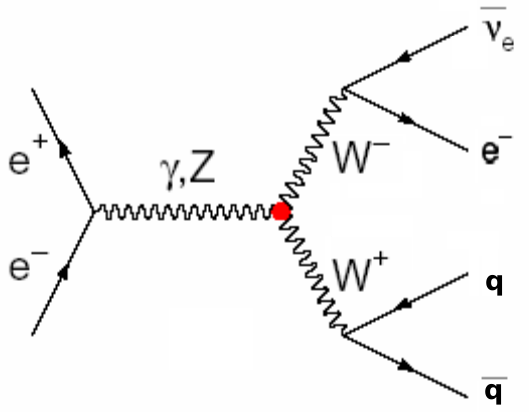
\includegraphics[width=0.25\textwidth]{triple_gauge_s_chan.png} \hspace{1em}
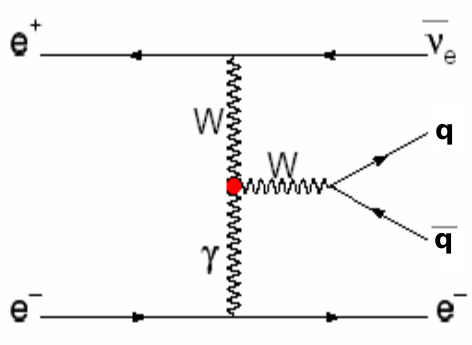
\includegraphics[width=0.25\textwidth]{triple_gauge_t_chan.png} \hspace{1em}
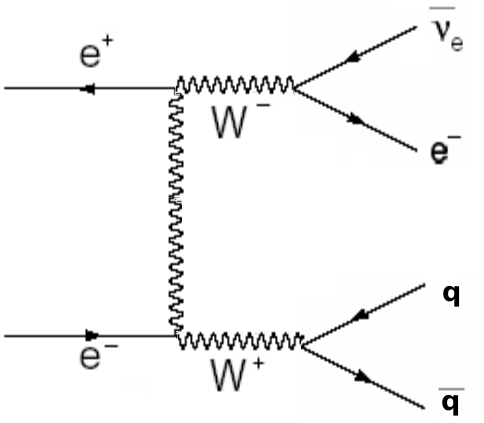
\includegraphics[width=0.25\textwidth]{triple_gauge_bkg.png}
\caption{
  The two main processes in \epm\ collisions for triple gauge couplings (marked in red) and the main background process.
}
\end{figure}

\end{frame}







\section{Analysis details}

\begin{frame}{Datasets}
\input{\texpath/samples.tex}
\vspace{-0.5cm}
The events in the datasets are scaled with the luminosity (1.5 \invab) and their \xsec.
%
Additionally, they are divided by the total number of entries in the dataset.
%
$W$ and $WW\rightarrow\qqln$ are separated by MC truth leptonic and hadronic \Wboson\ masses both be $< 100$~\GeV.
\end{frame}


\begin{frame}{Physics objects}
The physics objects used in this analysis are:
\begin{itemize}
  %
  \item Leptons
  \begin{itemize}
    \item Isolated leptons
  \end{itemize}
  %
  \item Jets
  \begin{itemize}
    \item use Pandora PFOs without isolated leptons
    \item reconstructed using the Valencia alrogithm\footnote{algorithm string in marlin: `ValenciaPlugin 0.8 1 0.7'} with
    \begin{itemize}
      \item jet size $R=0.8$
      \item clustering order $\beta=1.0$
      \item jet shrinking for forward jets $\gamma=0.7$
    \end{itemize}
  \end{itemize}
  %
  \item Missing energy
  \begin{itemize}
    \item Initial state minus sum of selected jets and lepton
  \end{itemize}
  %
\end{itemize}
\end{frame}










\section{Event selection}

\begin{frame}{Event selection}
A preliminary list of event selection cuts has been applied to select the \qqln\ final state:
\begin{itemize}
%
\item Pre-cut - an intermediate step to see separate effects
\begin{itemize}
\item Exactly one charged lepton
\item Exactly one muon (electrons are still undressed and left out for now)
\end{itemize}
%
\item Final - the preliminary full event selection
\begin{itemize}
\item The pre-cut selection
\item Remove events with forward jets by requiring $|\cos \theta| < 0.95$
\item Maximum total jet energy $< 750$~\GeV
\item Lepton $\pt > 30$~\GeV
\end{itemize}
%
\end{itemize}
\end{frame}









\section{Event yields}

\subsection{Single selection cuts}

\begin{frame}{Signal $WW\rightarrow\qqln$}
\input{\texpath/final_cut_signal_qqln.tex}
The relative efficiency of every selection cut is listed (`Single') as well as the total efficiency (`Total').
%
The number of entries and the scaled number of events, using the cross-section and luminosity, are shown as well.
\end{frame}

\begin{frame}{Background $W\rightarrow\qqln$}
\input{\texpath/final_cut_bkg_qqln.tex}
The relative efficiency of every selection cut is listed (`Single') as well as the total efficiency (`Total').
%
The number of entries and the scaled number of events, using the cross-section and luminosity, are shown as well.
\end{frame}

\begin{frame}{Background $WW\rightarrow\qqll$}
\input{\texpath/final_cut_bkg_qqll.tex}
The relative efficiency of every selection cut is listed (`Single') as well as the total efficiency (`Total').
%
The number of entries and the scaled number of events, using the cross-section and luminosity, are shown as well.
\end{frame}

\subsection{Final event yield}

\begin{frame}{Final event yield}
\input{\texpath/final_yield.tex}
\end{frame}












\section{Event selection figures}


\subsection{Events}

\begin{frame}{Beam energy}
\begin{figure}
\includegraphics[width=0.5\textwidth]{{\figurepath/raw_beam_e}.pdf}
\includegraphics[width=0.5\textwidth]{{\figurepath/raw_beam_m}.pdf}\\ \tripleFigDistance
\includegraphics[width=0.5\textwidth]{{\figurepath/pre_beam_e}.pdf}
\includegraphics[width=0.5\textwidth]{{\figurepath/pre_beam_m}.pdf}\\ \tripleFigDistance
\includegraphics[width=0.5\textwidth]{{\figurepath/fin_beam_e}.pdf}
\includegraphics[width=0.5\textwidth]{{\figurepath/fin_beam_m}.pdf}
\caption{
  \eplus\ \eminus\ beam energy and mass
}
\end{figure}
\end{frame}

\begin{frame}{MC truth \Wboson\ masses}
\begin{figure}
\includegraphics[width=0.5\textwidth]{{\figurepath/raw_mc_qq_m}.pdf}
\includegraphics[width=0.5\textwidth]{{\figurepath/raw_mc_ln_m}.pdf}\\ \tripleFigDistance
\includegraphics[width=0.5\textwidth]{{\figurepath/pre_mc_qq_m}.pdf}
\includegraphics[width=0.5\textwidth]{{\figurepath/pre_mc_ln_m}.pdf}\\ \tripleFigDistance
\includegraphics[width=0.5\textwidth]{{\figurepath/fin_mc_qq_m}.pdf}
\includegraphics[width=0.5\textwidth]{{\figurepath/fin_mc_ln_m}.pdf}
\caption{
  Masses of the two W objects at truth level.
}
\end{figure}
\end{frame}



\subsection{Missing energy}

\begin{frame}{Missing energy kinematics}
\begin{figure}
\includegraphics[width=0.5\textwidth]{{\figurepath/raw_miss_e}.pdf}
\includegraphics[width=0.5\textwidth]{{\figurepath/raw_miss_pt}.pdf}\\ \tripleFigDistance
\includegraphics[width=0.5\textwidth]{{\figurepath/pre_miss_e}.pdf}
\includegraphics[width=0.5\textwidth]{{\figurepath/pre_miss_pt}.pdf}\\ \tripleFigDistance
\includegraphics[width=0.5\textwidth]{{\figurepath/fin_miss_e}.pdf}
\includegraphics[width=0.5\textwidth]{{\figurepath/fin_miss_pt}.pdf}
\caption{
  Missing energy and \pt
}
\end{figure}
\end{frame}

\begin{frame}{Missing energy kinematics}
\begin{figure}
\includegraphics[width=0.5\textwidth]{{\figurepath/raw_miss_theta}.pdf}
\includegraphics[width=0.5\textwidth]{{\figurepath/raw_miss_phi}.pdf}\\ \tripleFigDistance
\includegraphics[width=0.5\textwidth]{{\figurepath/pre_miss_theta}.pdf}
\includegraphics[width=0.5\textwidth]{{\figurepath/pre_miss_phi}.pdf}\\ \tripleFigDistance
\includegraphics[width=0.5\textwidth]{{\figurepath/fin_miss_theta}.pdf}
\includegraphics[width=0.5\textwidth]{{\figurepath/fin_miss_phi}.pdf}
\caption{
  Missing energy $\phi$ and $\theta$
}
\end{figure}
\end{frame}




\subsection{Leptons}

\begin{frame}{All leptons}
\begin{figure}
\includegraphics[width=0.5\textwidth]{{\figurepath/raw_lep_n}.pdf}
\includegraphics[width=0.5\textwidth]{{\figurepath/raw_lep_type}.pdf}\\ \tripleFigDistance
\includegraphics[width=0.5\textwidth]{{\figurepath/pre_lep_n}.pdf}
\includegraphics[width=0.5\textwidth]{{\figurepath/pre_lep_type}.pdf}\\ \tripleFigDistance
\includegraphics[width=0.5\textwidth]{{\figurepath/fin_lep_n}.pdf}
\includegraphics[width=0.5\textwidth]{{\figurepath/fin_lep_type}.pdf}
\caption{
  Total lepton number and type
}
\end{figure}
\end{frame}

\begin{frame}{Total energy}
\begin{figure}
\includegraphics[width=0.5\textwidth]{{\figurepath/raw_lep_etot}.pdf}\\ \tripleFigDistance
\includegraphics[width=0.5\textwidth]{{\figurepath/pre_lep_etot}.pdf}\\ \tripleFigDistance
\includegraphics[width=0.5\textwidth]{{\figurepath/fin_lep_etot}.pdf}
\caption{
  Total lepton energy
}
\end{figure}
\end{frame}

\begin{frame}{Lepton kinematics}
\begin{figure}
\includegraphics[width=0.5\textwidth]{{\figurepath/raw_lep_e}.pdf}
\includegraphics[width=0.5\textwidth]{{\figurepath/raw_lep_pt}.pdf}\\ \tripleFigDistance
\includegraphics[width=0.5\textwidth]{{\figurepath/pre_lep_e}.pdf}
\includegraphics[width=0.5\textwidth]{{\figurepath/pre_lep_pt}.pdf}\\ \tripleFigDistance
\includegraphics[width=0.5\textwidth]{{\figurepath/fin_lep_e}.pdf}
\includegraphics[width=0.5\textwidth]{{\figurepath/fin_lep_pt}.pdf}
\caption{
  Lepton energy and \pt
}
\end{figure}
\end{frame}

\begin{frame}{Lepton kinematics}
\begin{figure}
\includegraphics[width=0.5\textwidth]{{\figurepath/raw_lep_theta}.pdf}
\includegraphics[width=0.5\textwidth]{{\figurepath/raw_lep_phi}.pdf}\\ \tripleFigDistance
\includegraphics[width=0.5\textwidth]{{\figurepath/pre_lep_theta}.pdf}
\includegraphics[width=0.5\textwidth]{{\figurepath/pre_lep_phi}.pdf}\\ \tripleFigDistance
\includegraphics[width=0.5\textwidth]{{\figurepath/fin_lep_theta}.pdf}
\includegraphics[width=0.5\textwidth]{{\figurepath/fin_lep_phi}.pdf}
\caption{
  Lepton $\phi$ and $\theta$
}
\end{figure}
\end{frame}


\begin{frame}{Electron kinematics}
\begin{figure}
\includegraphics[width=0.5\textwidth]{{\figurepath/raw_el_e}.pdf}
\includegraphics[width=0.5\textwidth]{{\figurepath/raw_el_pt}.pdf}\\ \tripleFigDistance
\includegraphics[width=0.5\textwidth]{{\figurepath/pre_el_e}.pdf}
\includegraphics[width=0.5\textwidth]{{\figurepath/pre_el_pt}.pdf}\\ \tripleFigDistance
\includegraphics[width=0.5\textwidth]{{\figurepath/fin_el_e}.pdf}
\includegraphics[width=0.5\textwidth]{{\figurepath/fin_el_pt}.pdf}
\caption{
  Electron energy and \pt
}
\end{figure}
\end{frame}

\begin{frame}{Electron kinematics}
\begin{figure}
\includegraphics[width=0.5\textwidth]{{\figurepath/raw_el_theta}.pdf}
\includegraphics[width=0.5\textwidth]{{\figurepath/raw_el_phi}.pdf}\\ \tripleFigDistance
\includegraphics[width=0.5\textwidth]{{\figurepath/pre_el_theta}.pdf}
\includegraphics[width=0.5\textwidth]{{\figurepath/pre_el_phi}.pdf}\\ \tripleFigDistance
\includegraphics[width=0.5\textwidth]{{\figurepath/fin_el_theta}.pdf}
\includegraphics[width=0.5\textwidth]{{\figurepath/fin_el_phi}.pdf}
\caption{
  Electron $\phi$ and $\theta$
}
\end{figure}
\end{frame}


\begin{frame}{Muon kinematics}
\begin{figure}
\includegraphics[width=0.5\textwidth]{{\figurepath/raw_mu_e}.pdf}
\includegraphics[width=0.5\textwidth]{{\figurepath/raw_mu_pt}.pdf}\\ \tripleFigDistance
\includegraphics[width=0.5\textwidth]{{\figurepath/pre_mu_e}.pdf}
\includegraphics[width=0.5\textwidth]{{\figurepath/pre_mu_pt}.pdf}\\ \tripleFigDistance
\includegraphics[width=0.5\textwidth]{{\figurepath/fin_mu_e}.pdf}
\includegraphics[width=0.5\textwidth]{{\figurepath/fin_mu_pt}.pdf}
\caption{
  Muon energy and \pt
}
\end{figure}
\end{frame}

\begin{frame}{Muon kinematics}
\begin{figure}
\includegraphics[width=0.5\textwidth]{{\figurepath/raw_mu_theta}.pdf}
\includegraphics[width=0.5\textwidth]{{\figurepath/raw_mu_phi}.pdf}\\ \tripleFigDistance
\includegraphics[width=0.5\textwidth]{{\figurepath/pre_mu_theta}.pdf}
\includegraphics[width=0.5\textwidth]{{\figurepath/pre_mu_phi}.pdf}\\ \tripleFigDistance
\includegraphics[width=0.5\textwidth]{{\figurepath/fin_mu_theta}.pdf}
\includegraphics[width=0.5\textwidth]{{\figurepath/fin_mu_phi}.pdf}
\caption{
  Muon $\phi$ and $\theta$
}
\end{figure}
\end{frame}




\subsection{Jets}

\begin{frame}{All jets}
\begin{figure}
\includegraphics[width=0.5\textwidth]{{\figurepath/raw_jet_n}.pdf}
\includegraphics[width=0.5\textwidth]{{\figurepath/raw_jet_etot}.pdf}\\ \tripleFigDistance
\includegraphics[width=0.5\textwidth]{{\figurepath/pre_jet_n}.pdf}
\includegraphics[width=0.5\textwidth]{{\figurepath/pre_jet_etot}.pdf}\\ \tripleFigDistance
\includegraphics[width=0.5\textwidth]{{\figurepath/fin_jet_n}.pdf}
\includegraphics[width=0.5\textwidth]{{\figurepath/fin_jet_etot}.pdf}
\caption{
  Total jet number and energy
}
\end{figure}
\end{frame}

\begin{frame}{Jet kinematics}
\begin{figure}
\includegraphics[width=0.5\textwidth]{{\figurepath/raw_jet_e}.pdf}
\includegraphics[width=0.5\textwidth]{{\figurepath/raw_jet_pt}.pdf}\\ \tripleFigDistance
\includegraphics[width=0.5\textwidth]{{\figurepath/pre_jet_e}.pdf}
\includegraphics[width=0.5\textwidth]{{\figurepath/pre_jet_pt}.pdf}\\ \tripleFigDistance
\includegraphics[width=0.5\textwidth]{{\figurepath/fin_jet_e}.pdf}
\includegraphics[width=0.5\textwidth]{{\figurepath/fin_jet_pt}.pdf}
\caption{
  Jet energy and \pt
}
\end{figure}
\end{frame}

\begin{frame}{Jet kinematics}
\begin{figure}
\includegraphics[width=0.5\textwidth]{{\figurepath/raw_jet_pt_0}.pdf}
\includegraphics[width=0.5\textwidth]{{\figurepath/raw_jet_pt_1}.pdf}\\ \tripleFigDistance
\includegraphics[width=0.5\textwidth]{{\figurepath/pre_jet_pt_0}.pdf}
\includegraphics[width=0.5\textwidth]{{\figurepath/pre_jet_pt_1}.pdf}\\ \tripleFigDistance
\includegraphics[width=0.5\textwidth]{{\figurepath/fin_jet_pt_0}.pdf}
\includegraphics[width=0.5\textwidth]{{\figurepath/fin_jet_pt_1}.pdf}
\caption{
  Leading and sub-leading jet \pt
}
\end{figure}
\end{frame}

\begin{frame}{Jet kinematics}
\begin{figure}
\includegraphics[width=0.5\textwidth]{{\figurepath/raw_jet_theta}.pdf}
\includegraphics[width=0.5\textwidth]{{\figurepath/raw_jet_phi}.pdf}\\ \tripleFigDistance
\includegraphics[width=0.5\textwidth]{{\figurepath/pre_jet_theta}.pdf}
\includegraphics[width=0.5\textwidth]{{\figurepath/pre_jet_phi}.pdf}\\ \tripleFigDistance
\includegraphics[width=0.5\textwidth]{{\figurepath/fin_jet_theta}.pdf}
\includegraphics[width=0.5\textwidth]{{\figurepath/fin_jet_phi}.pdf}
\caption{
  Jet $\phi$ and $\theta$
}
\end{figure}
\end{frame}





\subsection{Derived observables}

\begin{frame}{Invariant masses}
\begin{figure}
% \includegraphics[width=0.5\textwidth]{{\figurepath/raw_mjj}.pdf}\\ \tripleFigDistance
% \includegraphics[width=0.5\textwidth]{{\figurepath/pre_mjj}.pdf}\\ \tripleFigDistance
% \includegraphics[width=0.5\textwidth]{{\figurepath/fin_mjj}.pdf}
\includegraphics[width=0.5\textwidth]{{\figurepath/raw_mjj}.pdf}
\includegraphics[width=0.5\textwidth]{{\figurepath/raw_mln}.pdf}\\ \tripleFigDistance
\includegraphics[width=0.5\textwidth]{{\figurepath/pre_mjj}.pdf}
\includegraphics[width=0.5\textwidth]{{\figurepath/pre_mln}.pdf}\\ \tripleFigDistance
\includegraphics[width=0.5\textwidth]{{\figurepath/fin_mjj}.pdf}
\includegraphics[width=0.5\textwidth]{{\figurepath/fin_mln}.pdf}
\caption{
  Jet and charged lepton--neutrino invariant mass
}
\end{figure}
\end{frame}

\begin{frame}{Total event}
\begin{figure}
\includegraphics[width=0.5\textwidth]{{\figurepath/raw_mtot}.pdf}
\includegraphics[width=0.5\textwidth]{{\figurepath/raw_etot}.pdf}\\ \tripleFigDistance
\includegraphics[width=0.5\textwidth]{{\figurepath/pre_mtot}.pdf}
\includegraphics[width=0.5\textwidth]{{\figurepath/pre_etot}.pdf}\\ \tripleFigDistance
\includegraphics[width=0.5\textwidth]{{\figurepath/fin_mtot}.pdf}
\includegraphics[width=0.5\textwidth]{{\figurepath/fin_etot}.pdf}
\caption{
  Total invariant mass and energy of the event
}
\end{figure}
\end{frame}


% \section{Results}










\section{Lepton dressing}

\begin{frame}{Lepton dressing}
Electrons (and to a lesser extent) muons radiate photons as they traverse the detector. These photons are reconstructed as separate particles, while actually belonging to their mother electron. Clustering the photons in the vicinity of a lepton candidate helps recovering this energy which would otherwhise be lost. This improves the overall quality of the lepton reconstruction.

\vspace{1em}
The IsolatedLeptonFinder is being extended with an option to produce dressed leptons.
It can be set to either replace the regular lepton container or be produced in addition, for comparison and tuning.

\vspace{1em}
Status:
\begin{itemize}
\item the main functionality is implemented
\item lively discussion on \href{https://github.com/iLCSoft/MarlinReco/pull/33}{GitHub}.
\end{itemize}
\end{frame}









\section{Conclusion}

\begin{frame}{Conclusion}
The analysis of the \eeto\qqln channel is ongoing. The next steps are:
\begin{itemize}
\item rerun the analysis with updated missing energy (running as we speak)
\item refine the event selection (e.g. select high $\sqrt{s'}$ events)
\item determine differential cross-sections
\item estimate efficiencies
\end{itemize}


The lepton dressing is being implemented in ILCsoft. The next steps are:

\begin{itemize}
\item minimize the programmatical overhead of the new functionality
\item add sensible steering parameters and defaults
\end{itemize}


\vspace{1em}
Thank you for your attention, feedback is very welcome!
\end{frame}


% \appendix

% \section{Appendix}

% \begin{frame}{Event properties}
% \begin{figure}
% \includegraphics[width=0.5\textwidth]{{\figurepath/raw_sf}.pdf}\\ \tripleFigDistance
% \includegraphics[width=0.5\textwidth]{{\figurepath/pre_sf}.pdf}\\ \tripleFigDistance
% \includegraphics[width=0.5\textwidth]{{\figurepath/fin_sf}.pdf}
% \caption{
%   The applied scale factors
% }
% \end{figure}
% \end{frame}







\end{document}
